\documentclass[11pt,a4paper,oneside]{article}
\usepackage[a4paper,margin=1in]{geometry}
\usepackage[separate-uncertainty=true,range-phrase=--]{siunitx}
\usepackage[utf8]{inputenc}
\usepackage[T1]{fontenc}
\usepackage{mathtools}
\usepackage{amsfonts}
\usepackage{amsthm}
\usepackage{thmtools}
\usepackage{amssymb}
\usepackage{graphicx}
\usepackage{enumitem}
\usepackage[sfdefault]{roboto}
\usepackage[bibstyle=alphabetic,citestyle=alphabetic,natbib=false,backend=biber,sorting=nyt,hyperref=true,backref=true]{biblatex}
\usepackage[pdftex,hyperfootnotes=false,pdfpagelabels]{hyperref}
\usepackage{csquotes}
\usepackage[capitalise,noabbrev]{cleveref}
\usepackage{fancyhdr}
\usepackage{titlesec}
\usepackage{lipsum}
\usepackage{flafter}
\usepackage[x11names]{xcolor} 

\titleformat{name=\section}{\huge\bfseries\sffamily}{\rlap{\color{Aquamarine1!92!Chartreuse1}\rule[-0.4cm]{\linewidth}{1.2cm}} \thesection}{.5em}{}
\renewcommand{\headrulewidth}{0pt}

\title{OCNS Newsletter: Autumn 2024}
\author{OCNS members}
\date{\today}
\addbibresource{bibliography.bib}

\begin{document}
\pagestyle{fancy}
\fancyhead{}
\fancyfoot{}
\maketitle
\newpage

\pagestyle{fancy}
\fancyhead{}
\fancyfoot{}
\fancyfoot[L]{Volume 8 No 2}
\fancyfoot[C]{OCNS Newsletter}
\fancyfoot[R]{Page \thepage}

\newpage
\section*{Message from the President}%
\textbf{\large Thomas Nowotny, Professor of Informatics, University of Sussex, UK\\}
\rule{\textwidth}{0.4pt}

\lipsum[1-3]

\newpage
\section*{CNS 2024 Natal: Report from Local Organizer}%
\textbf{\large Cesar\\}
\rule{\textwidth}{0.4pt}
\lipsum[1-3]

\newpage
\section*{CNS 2024 Natal: Messages from Volunteers}%
\rule{\textwidth}{0.4pt}
\lipsum[1-3]

\newpage
\section*{CNS 2024 Natal: Travel Awards}%
\textbf{\large Michelle\\}
\rule{\textwidth}{0.4pt}
This year's travel awards were competitive, with many more excellent applicants than available funds.
We were pleased to award 19 travel grants to participants from all over the world.

\newpage
\section*{CNS 2024 Natal: Feedback form Summary}%
\rule{\textwidth}{0.4pt}
\begin{figure}[h]
  \centering
  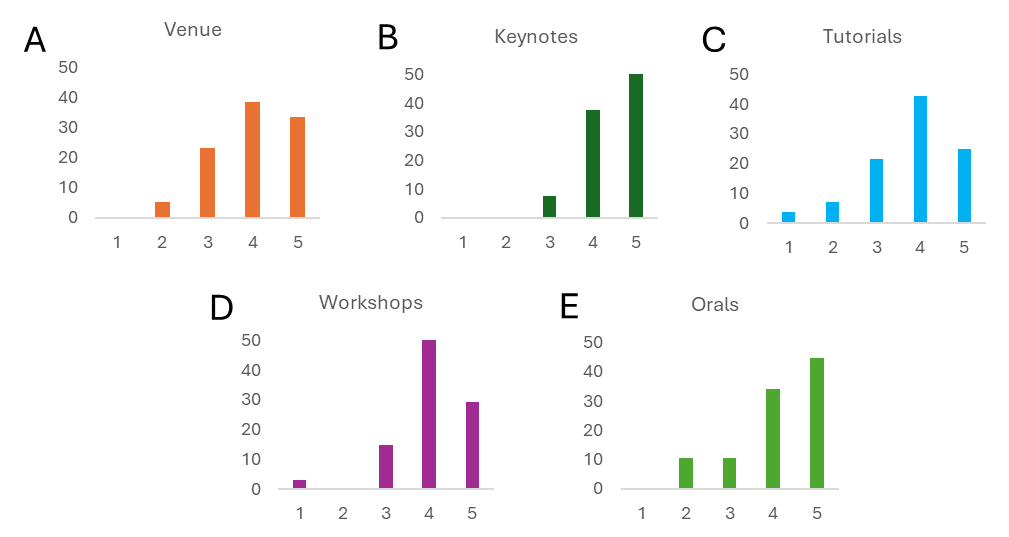
\includegraphics[width=\textwidth]{images/cns2024-feedback-form-summary}
  \caption{Summary of participant feedback, CNS*2024}%
  \label{fig:cns2024-summary}
\end{figure}

\noindent{}We received 42 responses on the Participant Feedback Survey distributed at the end of CNS*2024.
Overall, the feedback has been positive. The data is presented in \cref{fig:cns2024-summary} above, with 5 being the highest rating.

Most people have enjoyed the venue: 71\% gave 4 or 5 rating in this category (\cref{fig:cns2024-summary} A).
Attendees commented highly on the quality of the keynote speakers: 55\% gave the highest (5) rating in this category (\cref{fig:cns2024-summary} B).
The common theme was a commendation to the local organizers for catering, efficiency, and airport pickup; while the AV, staff English proficiency, and the small space allocated for posters received mostly negative comments.

Tutorials had mixed reviews: 10\% of the attendees submitted the rating less than average satisfaction (1 or 2), while most people, 42\%, gave the rating 4 (\cref{fig:cns2024-summary} C). No comments were provided.

The attendance at the workshops varied.
Some workshops received very high praise; 80\% of people gave ratings 4 or 5, with comments such as \enquote{very interesting topics}, \enquote{amazing}, \enquote{excellent session} (\cref{fig:cns2024-summary} D).
While other workshops left attendees dissatisfied, with suggestions to reduce the number of parallel sessions to boost the attendance.

Overall, 79\% attendees enjoyed oral presentations and gave the ratings 4 or 5, while 21\% rated the presentation as satisfactory (3) or below (2), \cref{fig:cns2024-summary} E.
Positive comments included \enquote{OCNS is superb in supporting young scientist's careers}.
Suggestions for improvements included more talks on data-driven, deep learning-based approaches.
We thank everybody for their feedback that will be taken into account when organizing CNS*2025.


\newpage
\section*{OCNS Initiatives: Software Working Group}%
\textbf{\large Marcel Stimberg \\
Ankur Sinha\\}
\rule{\textwidth}{0.4pt}
\lipsum[1-3]

\newpage
\section*{OCNS Initiatives: Mentoring Program Updates}%
\textbf{\large Eirini\\}
\rule{\textwidth}{0.4pt}
\lipsum[1-3]

\newpage
\section*{OCNS: New Program Committee}%
\textbf{\large Julie\\}
\rule{\textwidth}{0.4pt}
\lipsum[1-3]

\newpage
\section*{OCNS: Elections}%
%{\large Thomas Nowotny, Professor of Informatics, University of Sussex, UK\\}
\rule{\textwidth}{0.4pt}
\lipsum[1-3]

\newpage
\section*{CNS 2025 Florence}%
\textbf{\large ??\\}
\rule{\textwidth}{0.4pt}
\lipsum[1-3]

\newpage
\section*{OCNS: Member Updates}%
\rule{\textwidth}{0.4pt}
\lipsum[1-3]


\newpage
\section*{Messages from our Sponsors}%
\rule{\textwidth}{0.4pt}
\subsection*{Metacell}%
\begin{displayquote}
  Thank you to OCNS for hosting an excellent annual meeting, and to everyone who connected with MetaCell, attended our presentation and joined our event.
  It was great catching up with friends and partners in Natal, and we were proud sponsors of the meeting!

  If you're interested in new ways to standardize, visualize, share, and build your computational models, please visit \url{metacell.us} and get in touch with our team.
\end{displayquote}

\newpage
\section*{INCF Updates}%
\textbf{\large Helena/Matthew\\}
\rule{\textwidth}{0.4pt}
\lipsum[1-3]

\end{document}

